\chapter{第一部分}
\section{问题概述}
%
%%对问题的直观描述
%
该部分包含第1,2,3,4小题。

该部分要求使用各类搜索算法——DFS,BFS,UCS,$A^*$——来帮助吃豆人规划到达一处固定食物的路径。也就是说,要利用搜素算法寻找一条
从初始状态到目标状态的解路径,要确保每一步都是合法的,即遵循迷宫的约束。同时题目特别要求使用图搜索,以确保算法的完整性。

由于只有一处食物,该部分中的状态只需要包含吃豆人当前的位置即可,目标测试即判定当前位置是否与食物所在位置一致。

由于该部分中所需要的各类搜索算法,都遵循搜索算法的通用框架,唯一的区别在于从边缘队列中选取下一个展开结点的策略,因此
我先实现通用图搜索算法generalGraphSearch,然后实现各类从边缘队列中挑选结点的策略,从而达到实现各类搜索算法的目标。
%
%对项目已有代码的阅读和理解
%

%
%解决问题的思路和想法
%

\section{算法设计}
为了确保通用性,在generalGraphSearch中,我采用优先队列来实现边缘队列,并通过传入不同的优先性计算函数getPrioriy来实现不同的搜索算法。

由于题目要求的是图搜索算法,不同于树搜索和最佳优先算法,在generalGraphSearch中,如果一个结点已经被展开过,那么后续都不会再次被展开;
同时,展开获得的后继结点先不经检查便加入边缘序列中,直到依据特定策略从边缘序列中弹出后才检查是否已经被展开过,若没有,则展开。

下面给出的是generalGraphSearch的伪代码,其中getPriority是优先性计算函数。

\begin{procedure}[H]
    \SetKwFunction{getPriority}{getPriority}
    \SetKwFunction{getSolution}{getSolution}
    \SetKw{emptyActions}{emptyActions}
    \SetKw{in}{in}
    \SetKw{not}{not}
    \SetKw{continue}{continue}
    \KwOut{Actions}
    \lIf(\tcp*[h]{检查起始结点}){problem.isGoalState(problem.getStartState())}{\KwRet{\emptyActions}}
    初始化起始结点start\;
    初始化边缘队列frontier\tcp*[h]{采用优先队列}\;
    初始化reached表\tcp*[h]{采用字典}\;
    reached.add(start)\tcp*[h]{将start加入reached中}\;
    \lForEach(\tcp*[h]{添加start的所有后继}){child \in problem.getSuccessors(start)}{frontier.push(child,\getPriority(child))}
    \While{\not frontier.isEmpty()}
    {
        next = frontier.pop()\tcp*[h]{获取下一个展开结点}\;
        \lIf(\tcp*[h]{检查是否已访问过}){next \in reached}{\continue}
        reached.add(next)\tcp*[h]{将next加入reached中}\;
        \lIf(\tcp*[h]{通过目标检测}){problem.isGoalState(next)}{\KwRet{\getSolution(next,reached)}}
        \lForEach(\tcp*[h]{添加next的所有后继}){child \in problem.getSuccessors(next)}{frontier.push(child,\getPriority(child))}
    }
    \caption{generalGraphSearch(problem,getPriority)}
\end{procedure}

为了获取解序列,在通过目标检测后,需要从目标状态不断回溯至初始状态,同时保存其中所需要的动作。

\begin{procedure}
    \KwOut{Actions}
    初始化Actions\tcp*[h]{采用列表}\;
    cur = goal\tcp*[h]{初始化工作指针}\;
    \While(\tcp*[h]{起始节点无父节点}){reached[cur].parent}
    {
        solution.append(reached[cur].action)\tcp*[h]{添加到当前结点对应的动作}\;
        cur = reached[cur].parent\tcp*[h]{移动至父节点}\;
    }
    \KwRet{Actions.reverse()}\tcp*[h]{取反}
    \caption{getSolution(goal,reached)}
\end{procedure}

在generalGraphSearch的基础之上,只需定义特定的优先性计算函数,便能得到不同的图搜索算法。

在DFS和BFS算法中,一个结点的优先级和只它的深度有关。因为已有代码中提供的优先队列优先弹出优先级小的元素,所以
在DFS算法中当前结点的优先级应该比父节点要小;在BFS算法中当前结点的优先级应该比父节点要大。

\begin{function}[H]
    \SetKw{not}{not}
    \lIf(\tcp*[h]{无父节点,即起始结点}){\not parent}{\KwRet{0}}
    \KwRet{parent.priority-1}\tcp*[h]{优先级越小越优先}
    \caption{dfsPriority(parent)}
\end{function}

\begin{function}[H]
    \SetKw{not}{not}
    \lIf(\tcp*[h]{无父节点,即起始结点}){\not parent}{\KwRet{0}}
    \KwRet{parent.priority+1}\tcp*[h]{优先级越小越优先}
    \caption{bfsPriority(parent)}
\end{function}

在UCS算法中,一个结点的优先级和到该结点的路径的总代价相关。

\begin{function}[H]
    \SetKw{not}{not}
    \lIf(\tcp*[h]{无父节点,即起始结点}){\not parent}{\KwRet{0}}
    \KwRet{parent.priority+pathCost}\tcp*[h]{到父节点的总代价加上从父节点到该结点的代价}
    \caption{ucsPriority(parent,pathCost)}
\end{function}

在$A^*$算法中,一个结点的优先级不仅和到该结点的路径的总代价相关,也和启发式函数返回的值相关。

\begin{function}[H]
    \SetKw{not}{not}
    \SetKwFunction{heuristic}{heuristic}
    \lIf(\tcp*[h]{heuristic为给定的启发式函数}){\not parent}{\KwRet{\heuristic(state,problem)}}
    \KwRet{parent.priority+pathCost+\heuristic(state,problem)}
    \caption{AStarPriority(parent,pathCost,state)}
\end{function}

\begin{algorithm}[H]
    \KwRet{generalGraphSearch(problem,dfsPriority)}
    \caption{depthFirstSearch(problem)}
\end{algorithm}

\begin{algorithm}[H]
    \KwRet{generalGraphSearch(problem,bfsPriority)}
    \caption{breadthFirstSearch(problem)}
\end{algorithm}

\begin{algorithm}[H]
    \KwRet{generalGraphSearch(problem,ucsPriority)}
    \caption{uniformCostSearch(problem)}
\end{algorithm}

\begin{algorithm}[H]
    \KwRet{generalGraphSearch(problem,AStarPriority)}
    \caption{aStarSearch(problem)}
\end{algorithm}
%
%用自己的语言描述解决问题所使用的算法的原理及功能,设计思路和算法流程图
%

\section{算法实现}
%
%在算法原理的基础上,结合代码,讲述算法的实现细节、核心函数、模块输入输出,数据结构定义等内容
%
该部分中所需要的数据结构主要用于表示未展开的结点和已展开的结点。

对于已展开的结点,由于需要用于回溯形成解序列,所以需要存储父节点和行动,所以采用键值对形式,键为状态,值为对应的父节点和行动。
由于已展开的结点是由未展开的结点变化而来的,所以未展开的结点中也需要存储父节点和行动,除此之外,为了用于展开和计算子节点的相应性质,
还需要包含状态域、优先性域以及路径代价域。

\begin{lstlisting}
from typing import Callable, List, Dict, Tuple
from collections import namedtuple
from game import Stack, PriorityQueue
from game import Directions
#未展开结点
#用于展开结点,以及计算子节点的优先性和路径代价所以需要存储状态,优先性和路径代价
Node = namedtuple('Node',('state','pathCost','priority','property'))
Property = namedtuple('Property',('parent','action'))
#用于记录已访问结点,同时还要用于回溯形成解序列,所以需要存储父节点和行动,所以采用键值对形式,
Reached = Dict[Node.state,Property]
#行为
Action = (Directions.NORTH or Directions.SOUTH or
          Directions.EAST or Directions.WEST or
          Directions.LEFT or Directions.RIGHT or
          Directions.STOP or Directions.REVERSE)
Actions = List[Action]
\end{lstlisting}

由于字典要求键的类型可以进行散列,所以键中不能包含列表类型。因此,在将结点存放进Reached表中时,需要把用于作为键的状态域的
类型统一改为元组等可以进行散列的类型。为此,我编写了辅助函数list2tuple来将列表以及嵌套列表转换为元组和嵌套元组。这一转换在后续完成状态中包含
foodGrid的问题时是必要的,因为已有代码中使用嵌套列表来实现foodGrid。这一转换使得generalGraphSearch变得更加通用。

\begin{lstlisting}[emph={[3]state},emphstyle={[3]\color{vscode_parametercolor}}]
def list2tuple(state):
    if not isinstance(state, tuple):#如果是int等类型就直接返回
        return state
    return tuple(list2tuple(item) if isinstance(item, list) else item for item in state)#否则就遍历各个元素并判断
\end{lstlisting}

\begin{lstlisting}[emph={[3]problem,getPriority},emphstyle={[3]\color{vscode_parametercolor}},
    emph={[4]SearchProblem,Callable,Node,Actions,Reached},emphstyle={[4]\color{vscode_classcolor}}
    ]
def generalGraphSearch(problem: SearchProblem,
                       getPriority: Callable[[Node or None, float, Node.state], float]) -> Actions:
    if problem.isGoalState(problem.getStartState()):
        return []
    start = Node(problem.getStartState(), 0, getPriority(None, 0, problem.getStartState()), Property(None, None))
    frontier = PriorityQueue()
    reached: Reached = {list2tuple(problem.getStartState()): start.property}  # 初始化reached并添加初始结点
    for child in problem.getSuccessors(problem.getStartState()):
        state = list2tuple(child[0])
        frontier.push(Node(state, child[2], getPriority(start, child[2], state),Property(list2tuple(problem.getStartState()), child[1])),getPriority(start, child[2], state))  # 添加各子节点
    while not frontier.isEmpty():
        nextNode: Node = frontier.pop()  # 获取下一个待展开的结点
        if nextNode.state in reached.keys():  # 判断是否已展开
            continue
        reached[nextNode.state] = nextNode.property  # 标记为已展开
        if problem.isGoalState(nextNode.state):  # 目标检测
            return get_solution(nextNode.state, reached)
        for child in problem.getSuccessors(nextNode.state):
            state = list2tuple(child[0])
            new = Node(state, nextNode.pathCost + child[2], getPriority(nextNode, child[2], state),
                       Property(nextNode.state, child[1]))  # 初始化子节点
            frontier.push(new, new.priority)  # 添加各子节点
\end{lstlisting}

\begin{lstlisting}[emph={[3]goal,problem,getPriority,reached},emphstyle={[3]\color{vscode_parametercolor}},
    emph={[4]SearchProblem,Callable,Node,Actions,Reached},emphstyle={[4]\color{vscode_classcolor}}
    ]
def get_solution(goal: Node.state, reached: Reached) -> Actions:
    solution: Actions = []
    cur = goal
    while reached[cur].parent:
        solution.append(reached[cur].action)
        cur = reached[cur].parent
    return solution[::-1]  # 取反
\end{lstlisting}

由于测试用例要求实现的DFS搜索算法在处理边缘队列中的两个优先级相同的结点时优先弹出后加入的结点,而PriorityQueue则时优先弹出先加入的结点,为了避免改变
已有代码,我的处理方式是在每个结点的原有优先级基础上减少一个逐渐增加的小量,以避免出现优先级相同的情况。

\begin{lstlisting}[emph={[3]parent},emphstyle={[3]\color{vscode_parametercolor}},emph={[4]SearchProblem,Callable,Node,Actions,Reached},emphstyle={[4]\color{vscode_classcolor}}]
def cnt():
    i = 0
    while True:
        yield i
        i = i + 1

counter = cnt()

def dfsPriority(parent: Node or None, pathCost: float, state: Node.state) -> float:
    if not parent:
        return 0
    return parent.priority - 1 - next(counter) * epsilon  # 额外减少一个小量
\end{lstlisting}

\begin{lstlisting}[emph={[3]parent,pathCost},emphstyle={[3]\color{vscode_parametercolor}},emph={[4]SearchProblem,Callable,Node,Actions,Reached},emphstyle={[4]\color{vscode_classcolor}}]
def bfsPriority(parent: Node or None, pathCost: float, state: Node.state) -> float:
    if not parent:
        return 0
    return parent.priority + 1
\end{lstlisting}

\begin{lstlisting}[emph={[3]parent,pathCost},emphstyle={[3]\color{vscode_parametercolor}},emph={[4]SearchProblem,Callable,Node,Actions,Reached},emphstyle={[4]\color{vscode_classcolor}}]
def ucsPriority(parent: Node or None, pathCost: float, state: Node.state) -> float:
    if not parent:
        return 0
    return parent.priority + pathCost
\end{lstlisting}

我所设计的优先级计算函数的参数为父节点,路径代价和当前状态,以满足各种搜索算法的需求。
只需把上述三个优先级计算函数作为参数传入generalGraphSearch便可以得到所要的DFS,BFS,UCS算法。

\begin{lstlisting}[emph={[3]parent,pathCost,problem,heuristic,state},emphstyle={[3]\color{vscode_parametercolor}},emph={[4]SearchProblem,Callable,Node,Actions,Reached},emphstyle={[4]\color{vscode_classcolor}}]
def depthFirstSearch(problem: SearchProblem):
    return generalGraphSearch(problem, dfsPriority)

def breadthFirstSearch(problem: SearchProblem):
    return generalGraphSearch(problem, bfsPriority)

def uniformCostSearch(problem: SearchProblem):
    return generalGraphSearch(problem, ucsPriority)
\end{lstlisting}

在实现$A^*$算法时,需要使用到Python的高阶函数功能,因为启发式函数不能够作为参数传入我所设计的优先级计算函数中。
\begin{lstlisting}[emph={[3]parent,pathCost,problem,heuristic,state,position,goals},emphstyle={[3]\color{vscode_parametercolor}},emph={[4]SearchProblem,Callable,Node,Actions,Reached},emphstyle={[4]\color{vscode_classcolor}}]
def aStarSearch(problem: SearchProblem, heuristic=nullHeuristic):
    def AStarPriority(parent: Node or None, pathCost: float, state: Node.state) -> float:
        if not parent:
            return heuristic(problem.getStartState(), problem)
        return parent.pathCost + pathCost + heuristic(state, problem)

    return generalGraphSearch(problem, AStarPriority)
\end{lstlisting}
\section{实验结果}
%
%对试验结果进行详细展示,对每个问题展示测试截图,对于测试用例进行描述说明,对于为通过测试的用例结合自己的算法进行分析,可以结合调试过程进行分析
%
\subsection{Question1\&2}
成功通过Question1和Question2的全部测试,实验结果截图分别见图\ref{q1}和图\ref{q2}。Question1的测试针对实现的DFS算法,Question2针对的是BFS算法。
\begin{figure}[htbp]
    \centering
    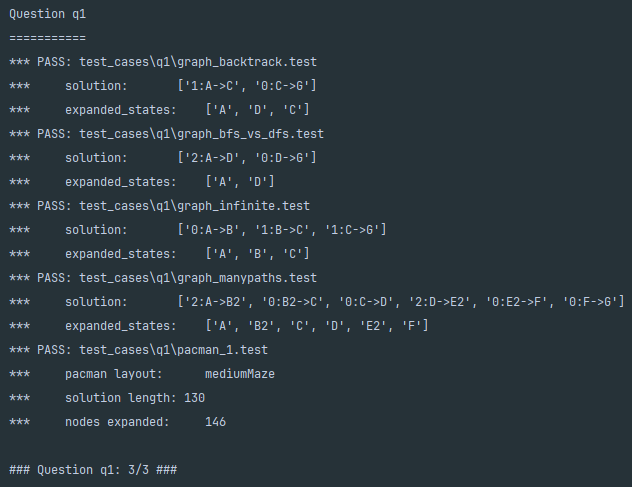
\includegraphics[scale = 0.7]{pic/q1.png}
    \caption{Question1实验结果}\label{q1}
\end{figure}
\begin{figure}[!htbp]
    \centering
    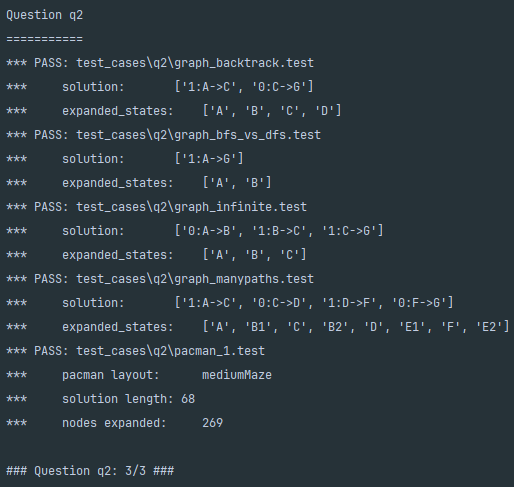
\includegraphics[scale = 0.7]{pic/q2.png}
    \caption{Question2实验结果}\label{q2}
\end{figure}

\begin{enumerate}
    \item {\bfseries graph\_backtrack:} 该测试用例旨在测试算法能否在简单情形下返回正确解路径。该测试样例中,cost并不都等于1,因此,实现DFS和BFS算法时不能够预设路径代价均为1,结点的优先级(深度)应该依据父节点的优先级(深度)进行计算。
    \item {\bfseries graph\_bfs\_vs\_dfs:}该测试用例旨在测试算法能否在简单情形下返回正确解路径,同时能够体现出DFS无法保证返回最优解的特性
    \item {\bfseries graph\_infinite:}该测试用例旨在测试算法能否在状态图存在回路的情况下返回正确解路径,generalGraphSearch中的reached表确保了算法不会陷入循环
    \item {\bfseries graph\_manypaths:}在该测试用例中,有多条解路径,因此同一结点可能会被放入边缘队列多次。cnt函数的使用确保了DFS算法解决优先级相同时的方法与答案一致,即后进边缘队列的结点先出队。
    \item {\bfseries pacman\_1:}该测试样例为吃豆人场景,迷宫大小为中等。可以看到,DFS展开的结点较少,但是返回的解路径较长;而BFS展开的结点较多,但是返回的解路径较短,实际上是最短的解路径。
\end{enumerate}
上述的测试样例中均有且仅有一个目标位置。
\subsection{Question3}
成功通过本问题的全部测试,实验结果截图见图\ref{q3}。
\begin{enumerate}
    \item {\bfseries graph\_backtrack,graph\_bfs\_vs\_dfs,graph\_infinite:}UCS在这三个测试样例中返回的解路径和展开的结点与BFS的均相同,但这只是人为设置而导致的巧合,在这些测试样例中路径代价并不全为1。
    \item {\bfseries ucs\_1\_problemC,ucs\_2\_problemE,ucs\_3\_problemW:}这三个测试样例共用同一个迷宫场景,吃豆人初始位置在右上角,目标位置有且仅有一个,在左下角。三个测试样例中的路径代价的特点分别为:始终为常数、沿东方向指数递减、沿西方向指数递减。由于目标位置在初始位置的西南方向,
    沿西方向递减的路径代价会诱导吃豆人朝目标探索,而沿东方向递减的路径代价则相反,因此前者对应的展开结点数量小于后者。但是由于迷宫的构造,前者所得到的解路径的长度却远大于后者。
    \item {\bfseries ucs\_4\_testSearch:}有两个目标位置,一个就紧邻着起始位置,但是对应的路径代价很高,另一个目标位置则相反。
    \item {\bfseries ucs\_5\_goalAtDequeue:}有且仅有一个目标位置,但有两条解路径,且会出现有两个目标结点同时出现在边缘队列的情况,先加入的路径代价更高。通过上述两个测试的关键在于目标检测只在一个结点离开边缘队列是进行。
\end{enumerate}
\begin{figure}[!htbp]
    \centering
    \begin{minipage}[t]{0.3\textwidth}
    \centering
    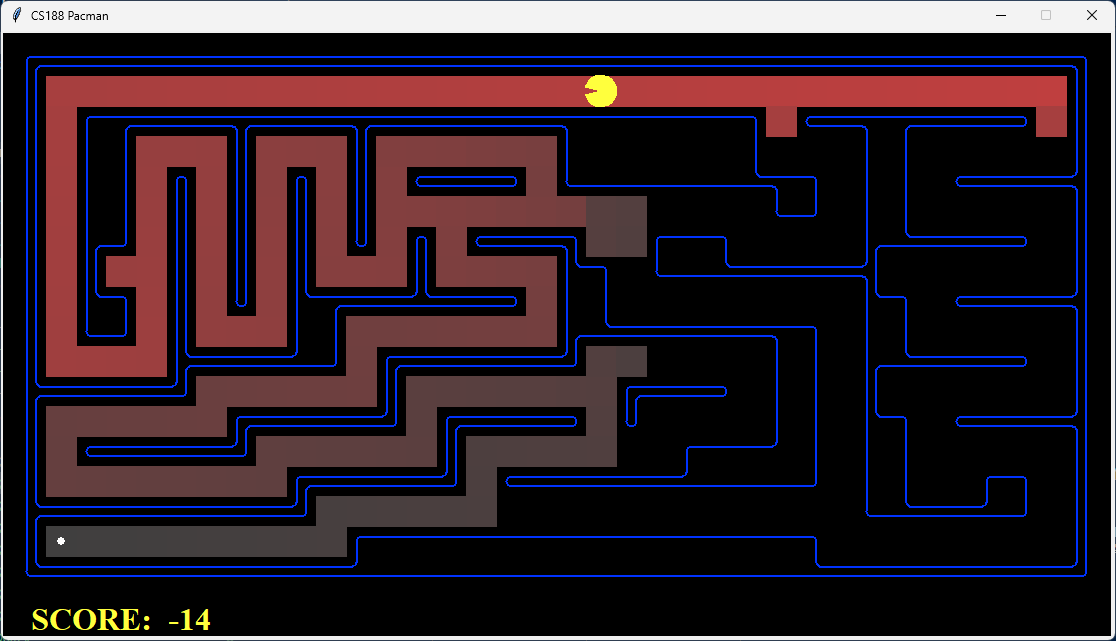
\includegraphics[width=\textwidth]{pic/W.png}
    \caption{ucs\_3\_problemW}\label{W}
    \end{minipage}
    \begin{minipage}[t]{0.3\textwidth}
    \centering
    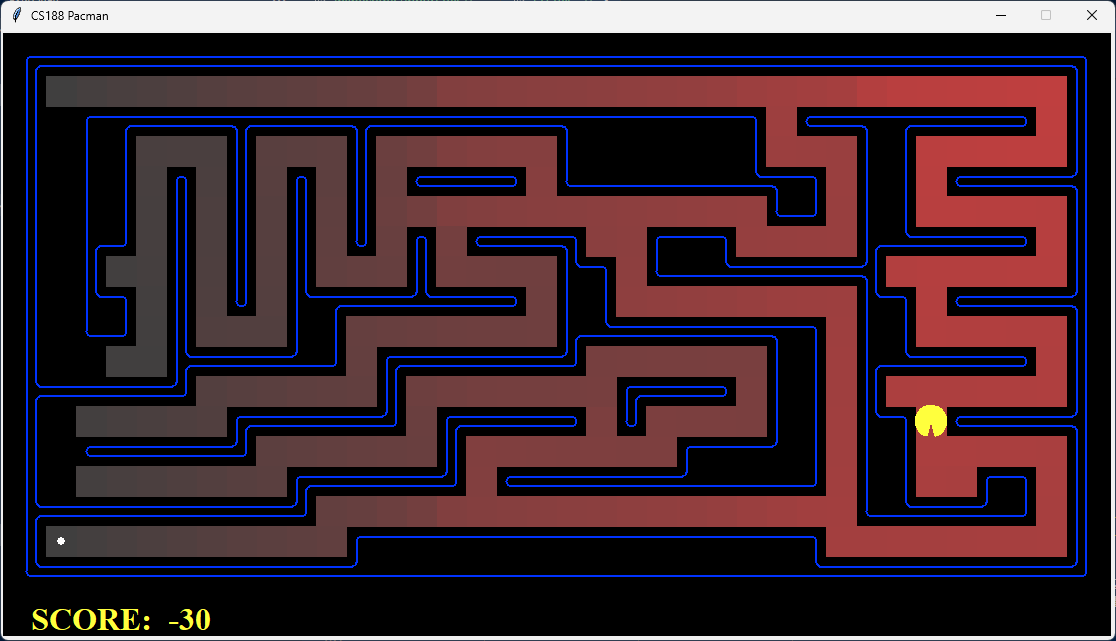
\includegraphics[width=\textwidth]{pic/E.png}
    \caption{ucs\_3\_problemE}\label{E}
    \end{minipage}
\end{figure}
\begin{figure}[!htbp]
    \centering
    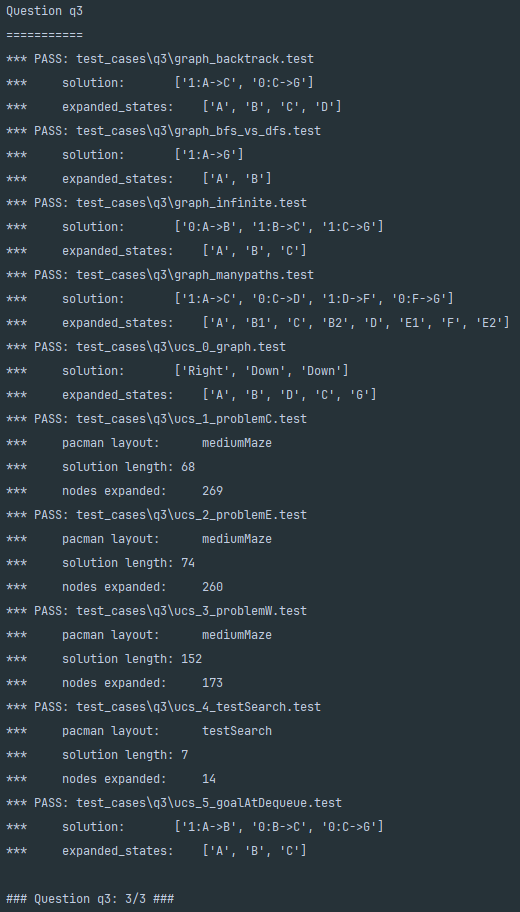
\includegraphics[width=0.7\textwidth]{pic/q3.png}
    \caption{Question3实验结果}\label{q3}
\end{figure}
\subsection{Question4}
成功通过本问题的全部测试,实验结果截图见图\ref{q4}。
\begin{figure}[!htbp]
    \centering
    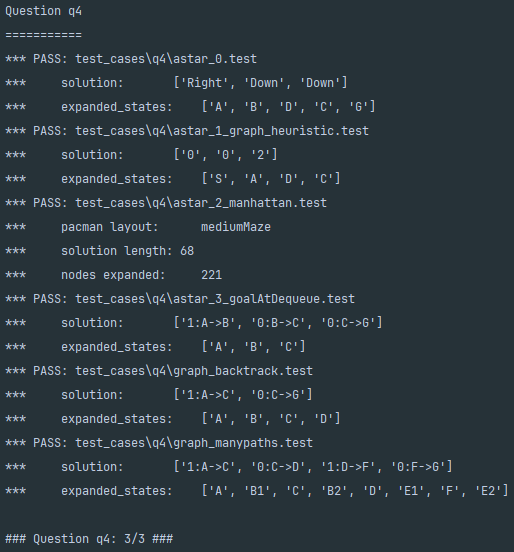
\includegraphics[width=0.7\textwidth]{pic/q4.png}
    \caption{Question4实验结果}\label{q4}
\end{figure}
\begin{enumerate}
    \item {\bfseries astar\_0:}该测试样例中包含两个目标结点,启发式函数恒为0,所设置的路径代价会使得算法无法给出解路径
    \item {\bfseries astar\_1\_graph\_heuristic:}有且仅有一个目标结点,要求算法进行图搜索
    \item {\bfseries astar\_2\_manhattan:}在迷宫环境中以曼哈顿距离为启发式函数
    \item {\bfseries astar\_3\_goalAtDequeue:}有且仅有一个目标位置,但有两条解路径,且会出现有两个目标结点同时出现在边缘队列的情况,先加入的路径代价更高。通过上述两个测试的关键在于目标检测只在一个结点离开边缘队列是进行。
    \item {\bfseries graph\_backtrack:}同之前的同名测试
    \item {\bfseries graph\_manypaths:}同之前的同名测试
\end{enumerate}
%
%实验中遇到的问题及解决方案,收获和思考:对算法的理解、优缺点的评价、算法的适用场景
%
